
\documentclass{beamer}
\DeclareGraphicsExtensions{.jpg, .pdf,.png,.eps}
\setbeamertemplate{caption}{\raggedright\insertcaption\par}

\usepackage{graphicx}
\title{MC-Cons}
\author{Gabriel Parent}



\usetheme{Execushares}

\begin{document}

\maketitle

\begin{frame}
	\frametitle{outline}
	\begin{center}
		\begin{itemize}
			\item background
			\item RNA consensus
			\item MC-Cons
			\item future work
		\end{itemize}
	\end{center}
\end{frame}


\section{background}

\begin{frame}
	\frametitle{many representations}
	\begin{figure}[!htb]
	\centering
	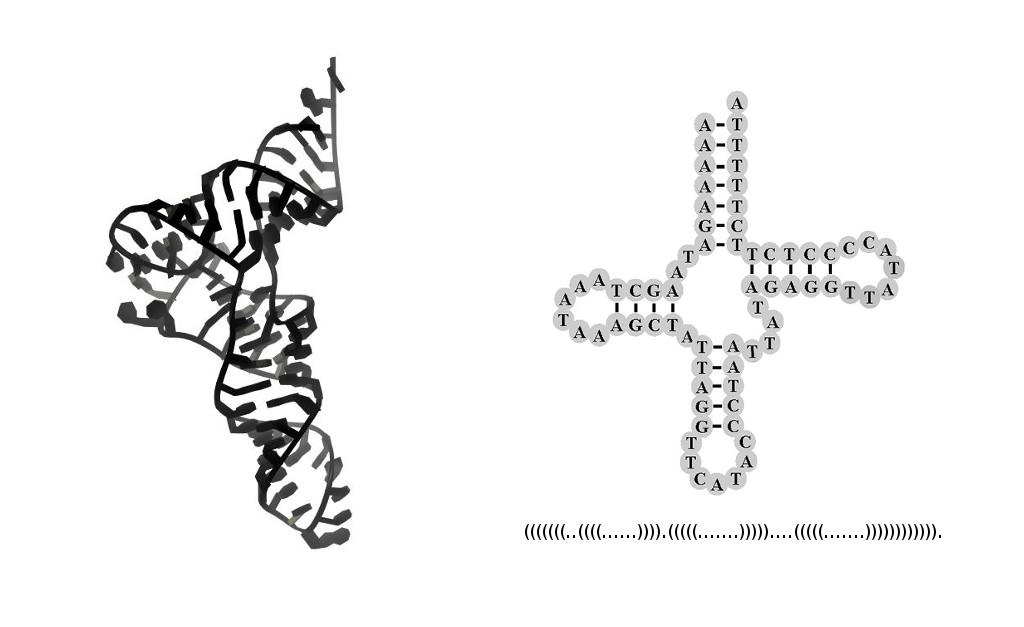
\includegraphics[scale=0.3]{figs/representations}
	%\caption{there are lots of ways to represent structure}
	\end{figure} 
\end{frame}



\begin{frame}
	\frametitle{many structures}
	\begin{figure}
	\centering
	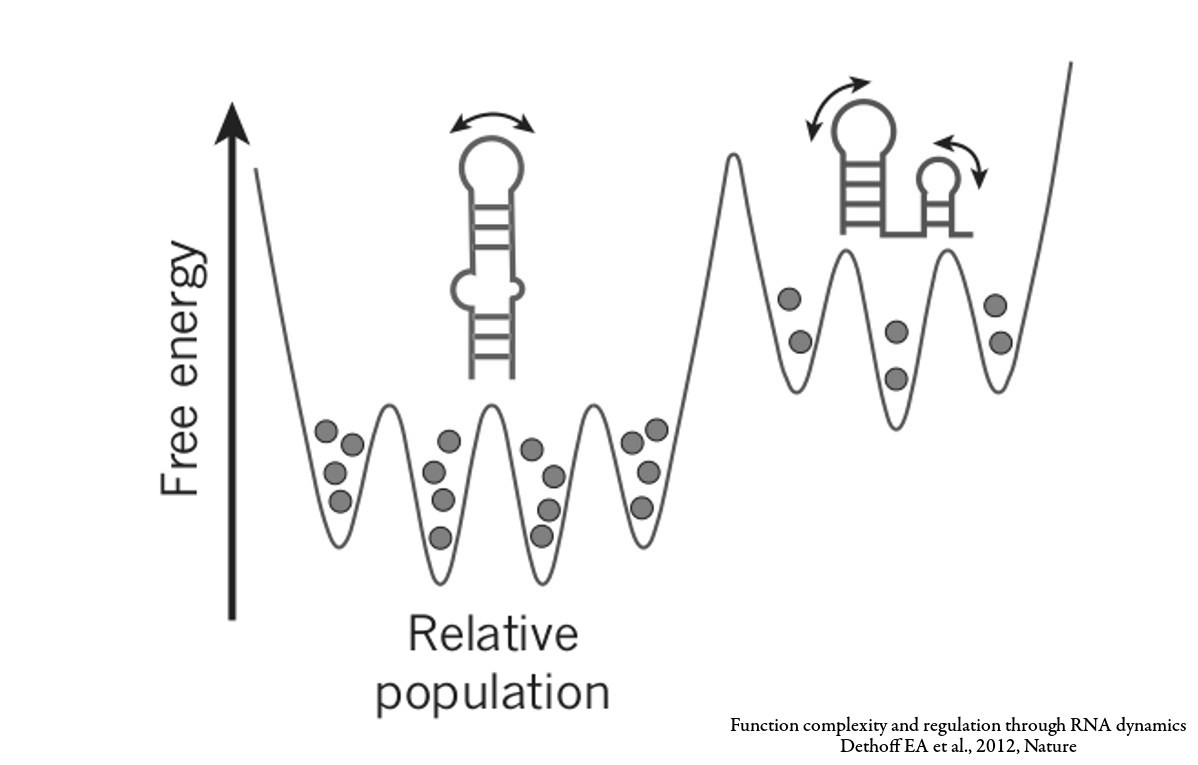
\includegraphics[scale=0.85]{figs/dynamics}
	%\caption{a single RNA molecule is present in many states}
	\end{figure}
\end{frame}


\begin{frame}
	\frametitle{many suboptimals}
	\begin{figure}
	\centering
	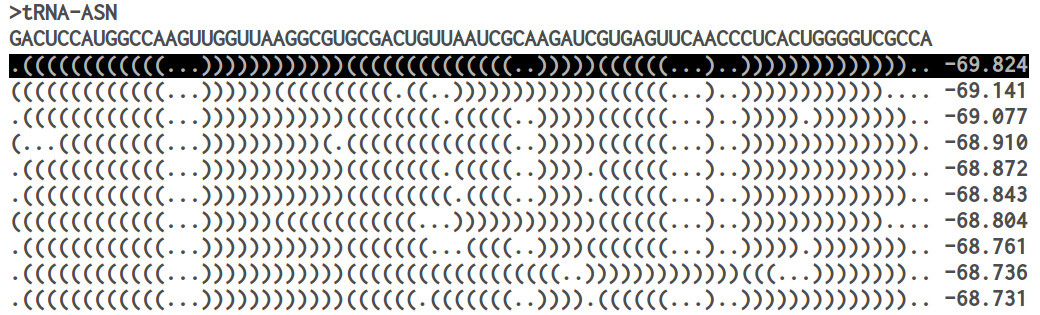
\includegraphics[scale=0.3]{figs/subopts}
	%\caption{many good potential structures}
	\end{figure}
\end{frame}




\section{RNA consensus}

\begin{frame}
	\frametitle{what we want}
	\begin{figure}
	\centering
	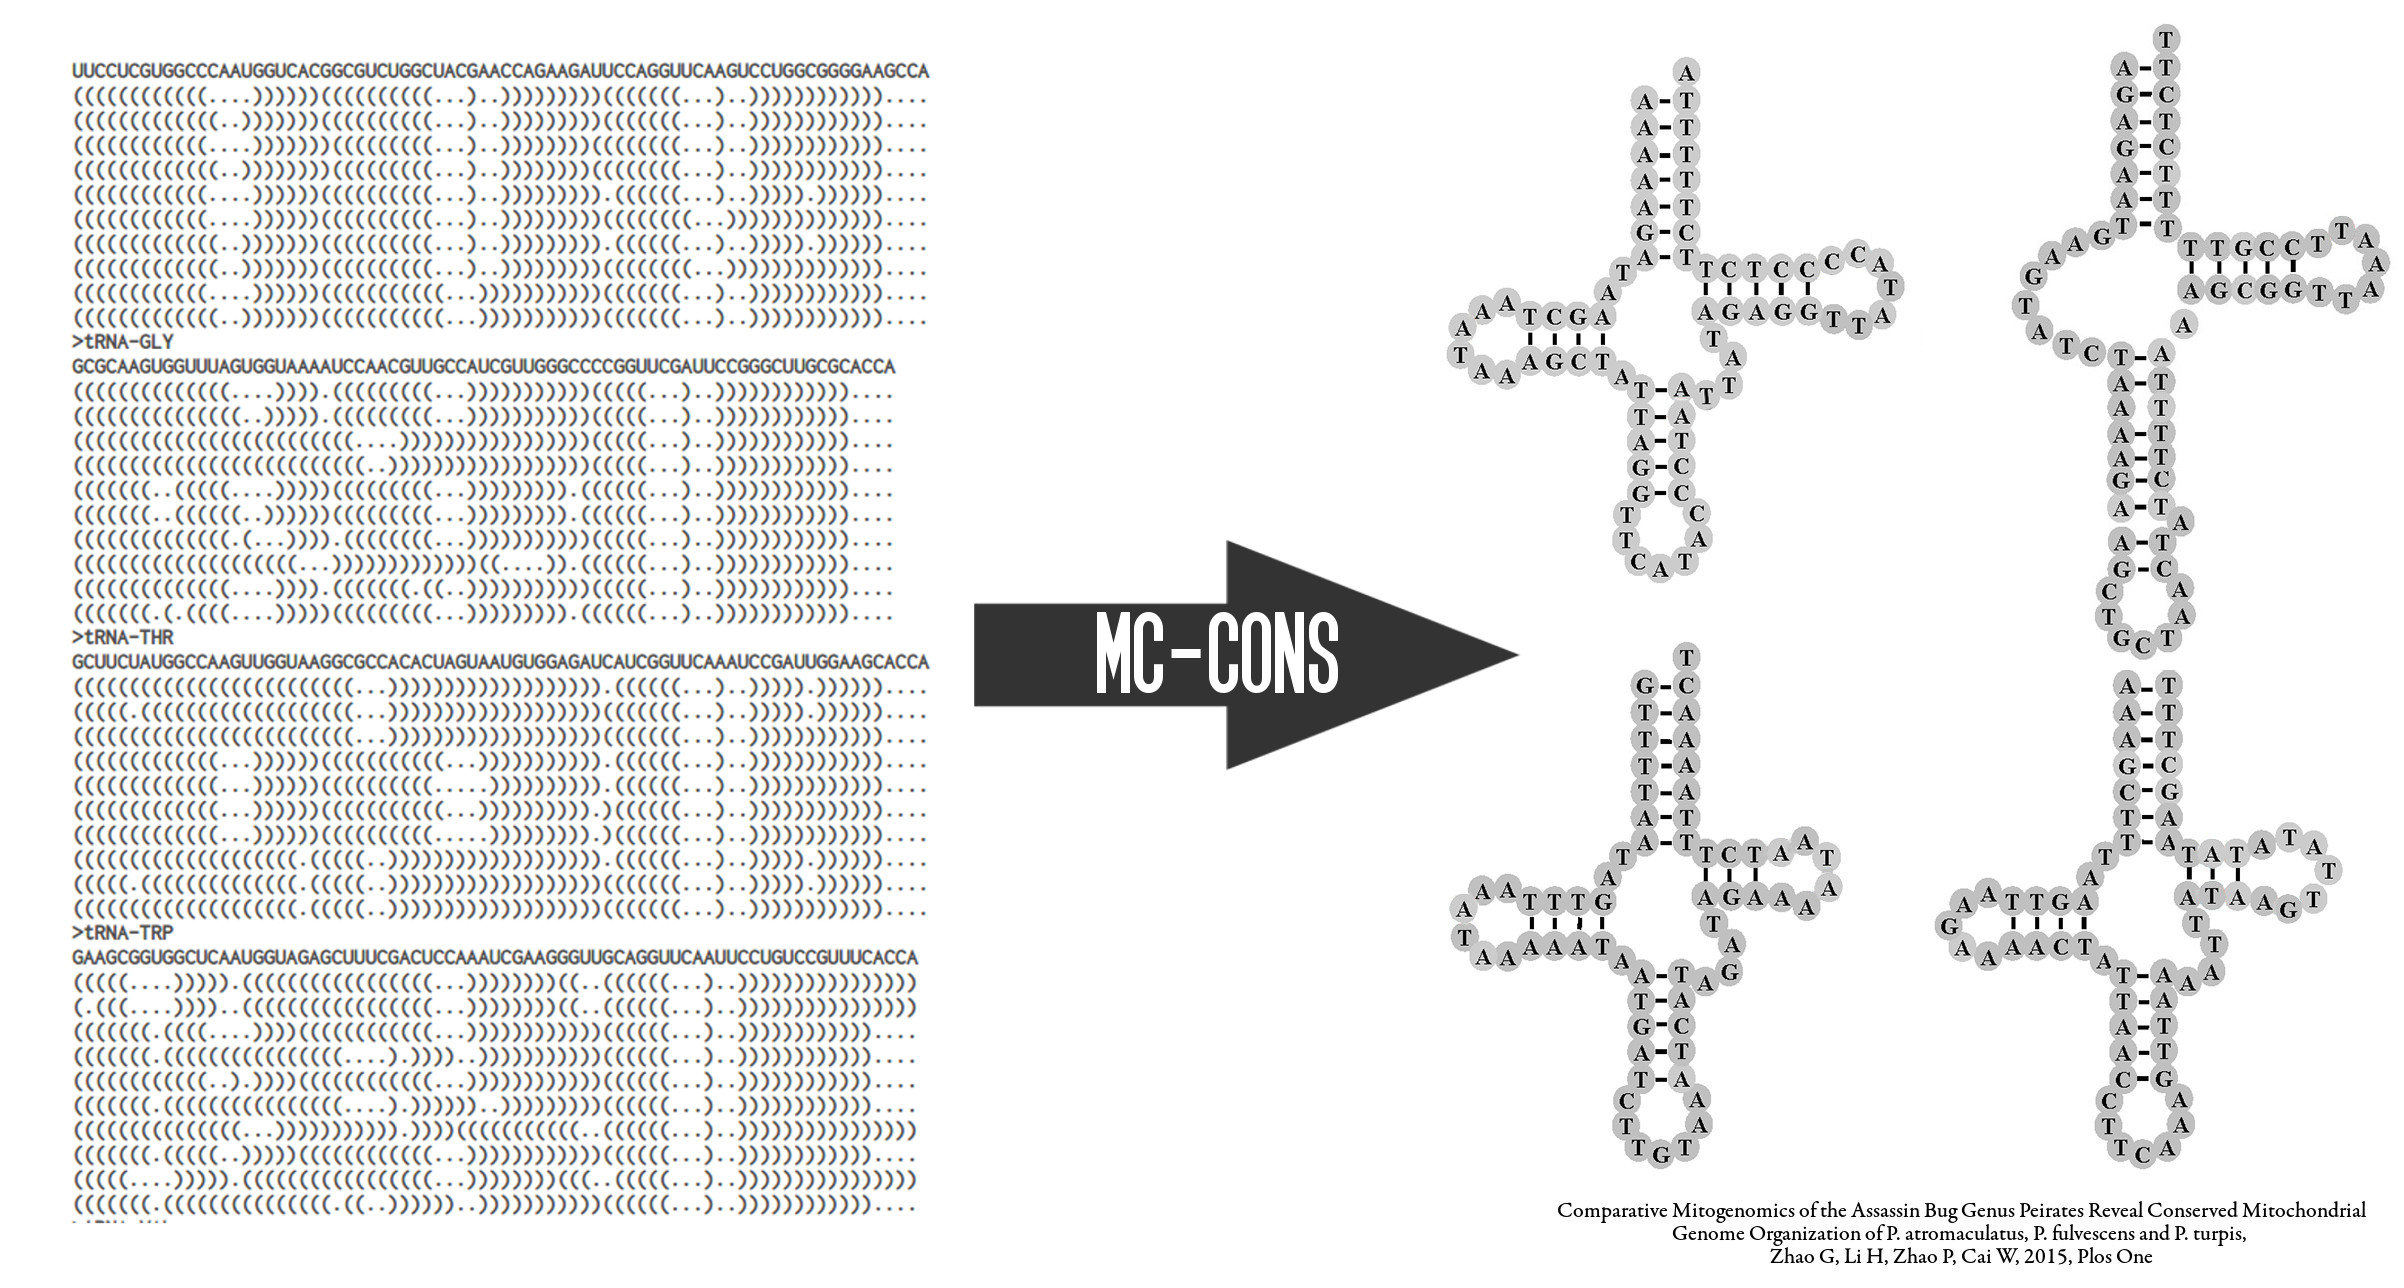
\includegraphics[scale=0.7]{figs/problem_setting}
	%\caption{}
	\end{figure}
\end{frame}



\section{MC-Cons}


\begin{frame}
	\frametitle{the approach}

	\begin{figure}
		\centering
		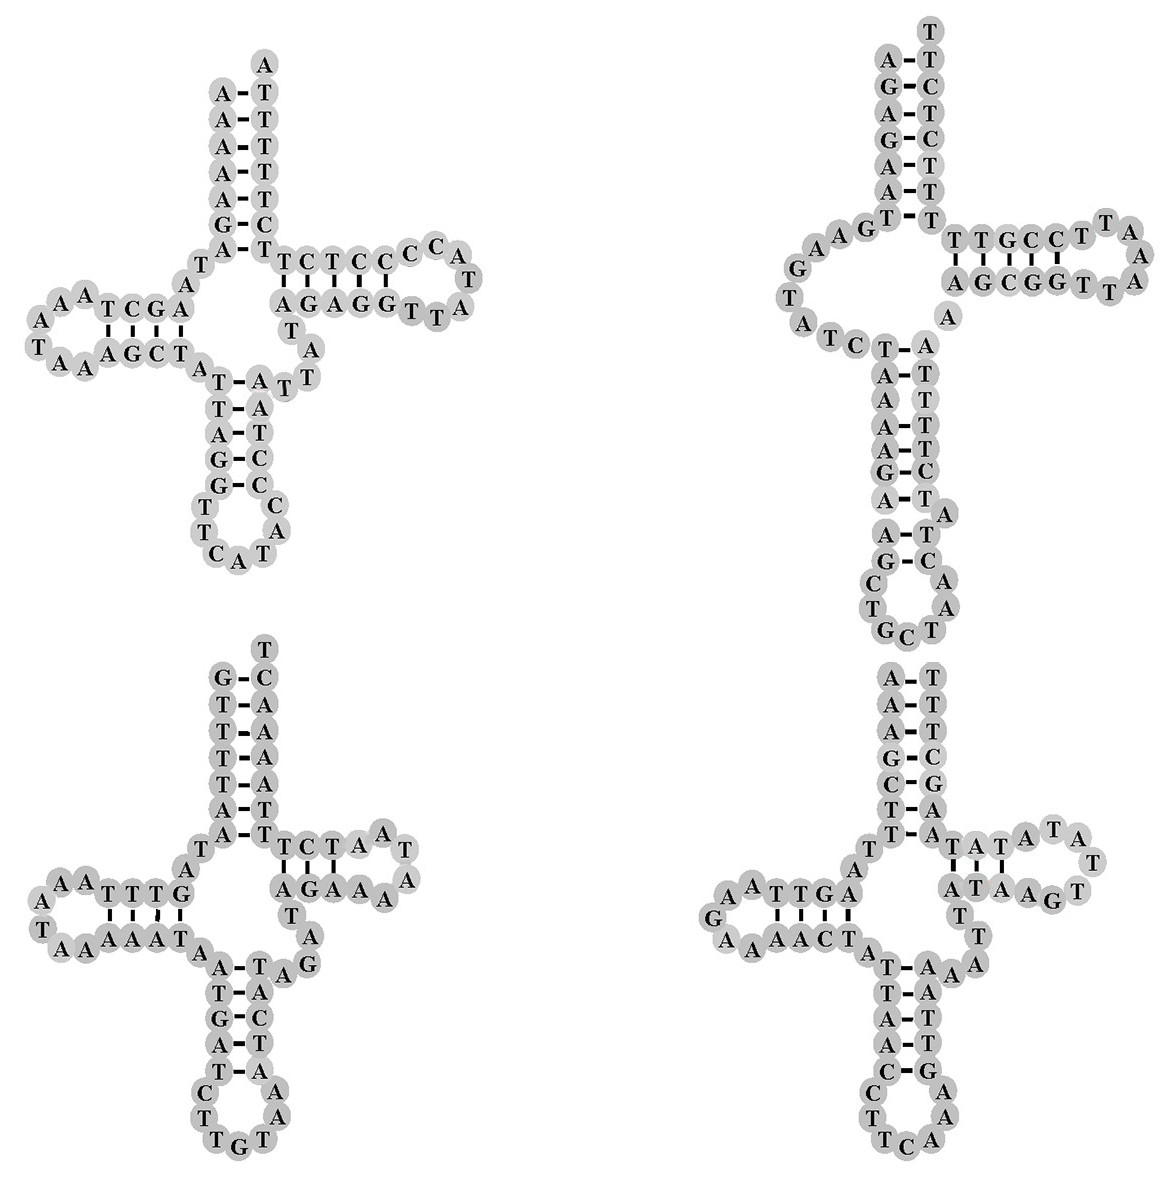
\includegraphics[scale=0.5]{figs/consensus}
	\end{figure}
	
	\begin{itemize}
		\item find pertinent distance function(s)		
		\item minimize the sum of pairwise distances
	\end{itemize}
	\begin{figure}
	\centering
	
	\end{figure}
\end{frame}



\begin{frame}
	\frametitle{how hard is this?}

	\begin{figure}
	\centering
	
\includegraphics[scale=0.4]{figs/np-complete}
	%\caption{}
	\end{figure}
	
\end{frame}


\begin{frame}
	\frametitle{good enough}
	\begin{figure}
	\centering
	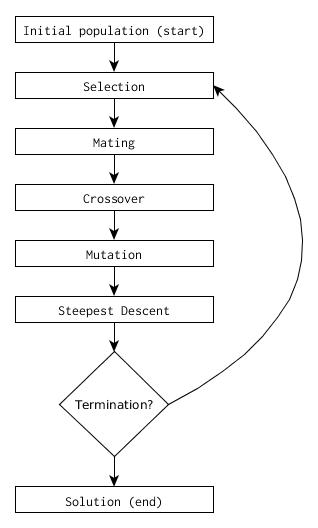
\includegraphics[scale=0.35]{figs/genetic_algorithm}
	%\caption{}
	\end{figure}
	
\end{frame}



\begin{frame}
	\frametitle{example: IREs}
	\begin{figure}
	\centering
	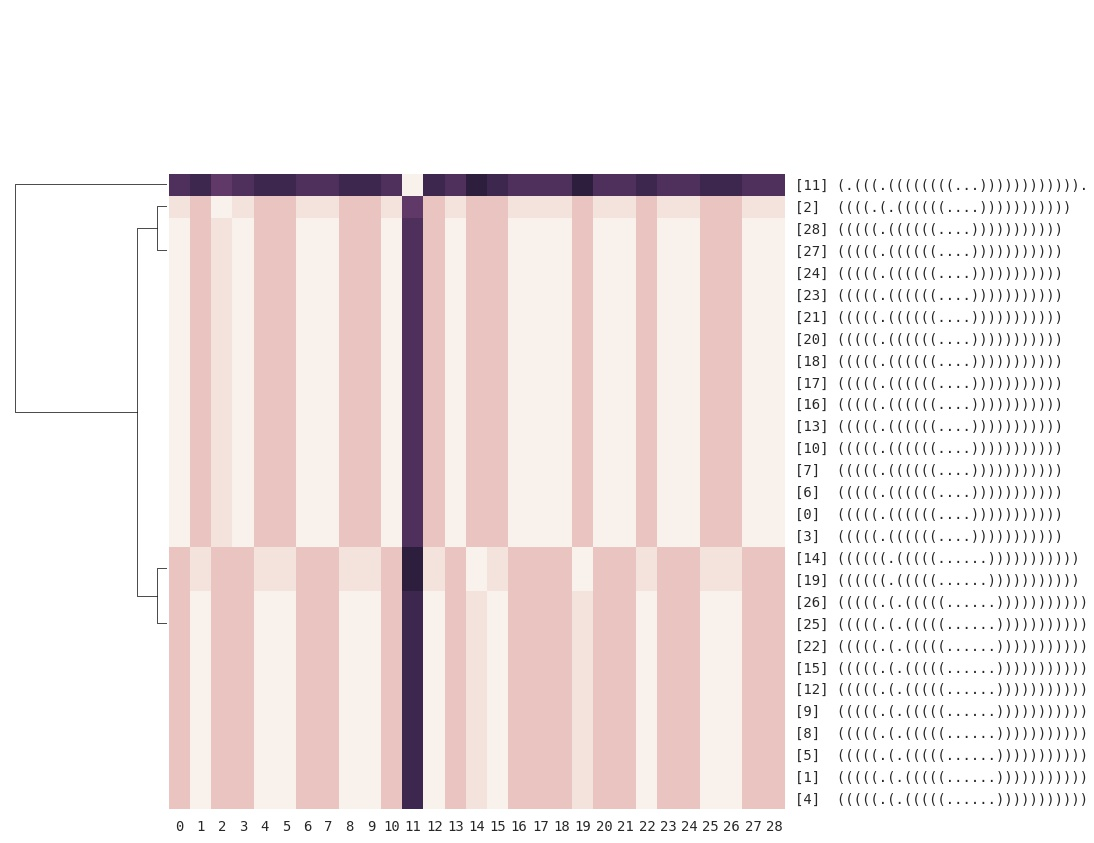
\includegraphics[scale=0.22]{figs/ires}
	%\caption{}
	\end{figure}
	
\end{frame}



\begin{frame}
	\frametitle{example: microRNAs}
%	\begin{figure}
%	\centering
%	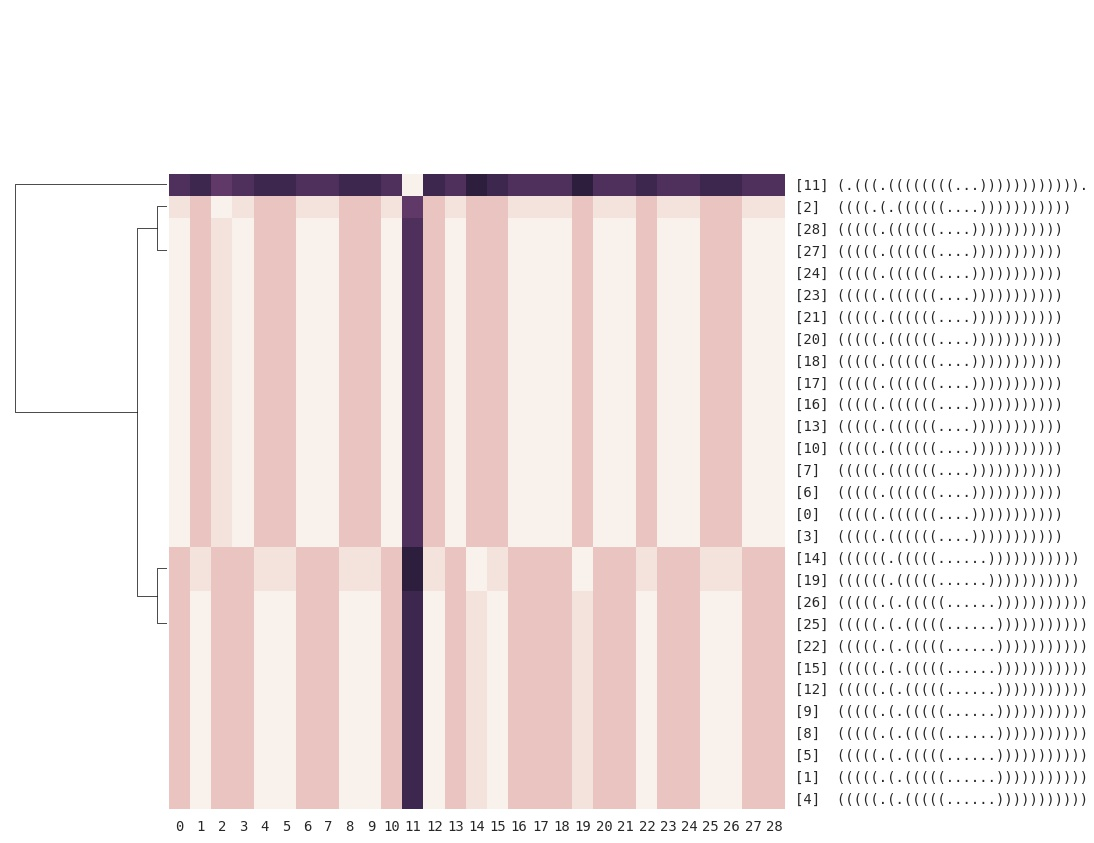
\includegraphics[scale=0.22]{figs/ires}
%	%\caption{}
%	\end{figure}
	
\end{frame}


\section{future work}
\begin{frame}
	\frametitle{future work}
	\begin{itemize}
		\item multi-objective option
		\item new distance functions
		\item parallelism
		\item user feedback (learning)
	\end{itemize}
\end{frame}


\begin{frame}
	\frametitle{questions}
	\begin{figure}
	\centering
	
\includegraphics[scale=1]{figs/beer}
	%\caption{}
	\end{figure}
	
\end{frame}


% TODO add slide for distance functions




%\begin{frame}
%	\frametitle{now you can have consensus!}
%	\begin{figure}[!htb]
%	\centering
%	\resizebox{0.75\textwidth}{!}{\input{consensus_example.pdf_tex}}
%	\caption{Let's suppose that their function is explained by a subset of similar structures (consensus). \\\hspace{\textwidth}In this case, 2 consensus make sense. Sometimes you get more, sometimes you get less.}
%	\end{figure} 
%\end{frame}

%
%
%\section{why?}
%
%\begin{frame}
%	\frametitle{what's the point?}
%\begin{figure}[!htb]
%\centering
%\resizebox{0.55\textwidth}{!}{\input{consensus_banner.pdf_tex}}
%\end{figure} 
%
%	\begin{itemize}
%		
%		\item goal: finding common/similar structures within suboptimal secondary structures
%		\item useful for
%		\begin{itemize}
%			\item improving secondary structure prediction for functionally related RNAs
%			\item exploring shared alternative structures
%		\end{itemize}
%	\end{itemize}
%	
%\end{frame}
%
%
%\section{how?}
%
%\subsection{general workflow}
%\begin{frame}
%	\frametitle{workflow}
%	\begin{columns}
%		\column{0.38\linewidth}
%		\centering
%		\begin{figure}[!htb]
%			\resizebox{1.\textwidth}{!}{\input{workflow.pdf_tex}}
%		\end{figure} 
%        
%        \column{0.58\linewidth}
%        \begin{itemize}
%        		\item a consensus minimizes the sum of pairs of distances between objects
%        		\item optimization steps
%        		\begin{enumerate}
%        		        			\item base pair structural similarity (modified tree edit distance)
%        			\item string edit distance on Vienna dot-bracket representation
%        		\end{enumerate}
%			\item two solver in C++ (branch \& bound and genetic algorithm)
%        \end{itemize}
%         \end{columns}
%         
%\end{frame} 
%
%
%\subsection{matching base pairs}
%\begin{frame}
%	\frametitle{first match base pairs}
%	\begin{figure}[!htb]
%	\centering
%	\resizebox{0.4\textwidth}{!}{\input{bp_tree.pdf_tex}}
%	\end{figure} 
%	
%	\begin{itemize}
%		\item base pair trees created (many-to-one function)
%		\item unit tree indel distance calculates number of base pairs to add or remove to transform a tree into another
%	\end{itemize}
%	
%
%\end{frame}
%
%
%
%\subsection{match the bulges}
%\begin{frame}
%	\frametitle{then match unpaired}
%	\begin{figure}[!htb]
%	\centering
%	\resizebox{0.75\textwidth}{!}{\input{tree_filtering.pdf_tex}}
%	\end{figure}	
%	\begin{itemize}
%		\item filtered by tree structure, now refine
%		\item placing the bulges around the skeleton...
%		\item string edit distance on dot-bracket
%	\end{itemize}
%\end{frame}
%
%
%
%\section{examples}
%\subsection{IREs}
%\begin{frame}
%	\frametitle{IREs}
%	\begin{figure}[!htb]
%	\centering
%	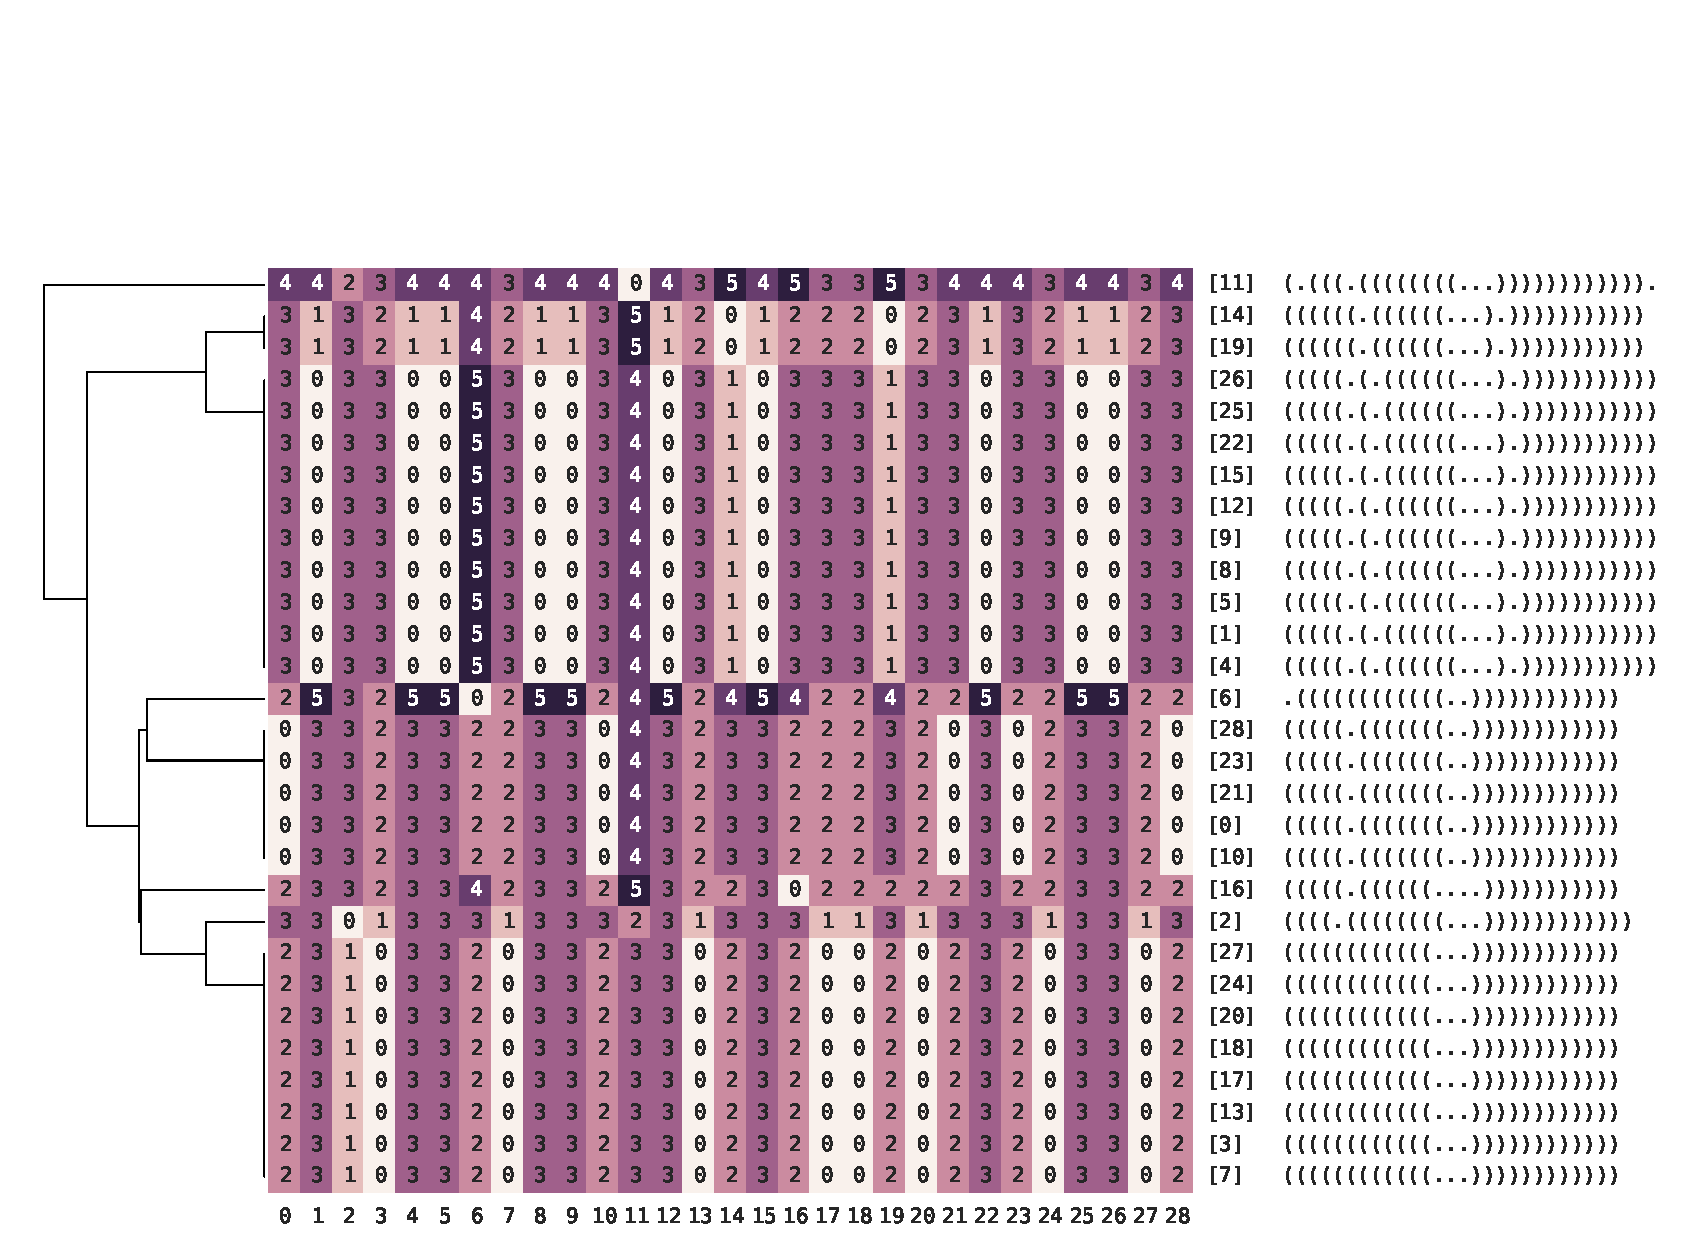
\includegraphics[scale=0.25]{figs/ires10.eps}
%	\caption{IREs structural assignment given 50 suboptimal for 29 different IREs.}
%	\end{figure} 
%\end{frame}
%
%
%
%\subsection{tRNAs}
%\begin{frame}
%	\frametitle{tRNAs}
%	
%
%\end{frame}
%
%

%
%
%
%\section{recap}
%
%\begin{frame}
%	\frametitle{recap}
%	\begin{itemize}
%		\item MC-Cons creates RNA 2D structural assignment
%		\item useful for finding structures explaining function
%		\item available at \url{https://github.com/major-lab/MC-Cons}
%	\end{itemize}
%\end{frame}
%
%\section{Q\&A}
%
%\begin{frame}
%	\frametitle{Q\&A}
%		\url{https://github.com/major-lab/MC-Cons}
%\end{frame}




\end{document}